\documentclass[dutch, a4paper, 11pt]{article}
\usepackage[utf8]{inputenc}

%Margins 
\usepackage[a4paper, left=1.27cm,top=1.27cm,right =1.27cm, bottom = 1.4cm]{geometry}

%Load packages
%Algemene packages
\usepackage{babel}
\usepackage{slantsc}
\usepackage{array}
\renewcommand{\arraystretch}{2}
\usepackage{multicol}
\usepackage{multirow}
\usepackage{amsmath}
\usepackage{amssymb}
\usepackage{amsfonts}
\usepackage{booktabs}


%Opsommingen
\usepackage{enumerate}


%Afbeeldingen
\usepackage{graphicx}
\usepackage{wrapfig}

%Gekleurde tekstboxen 
\usepackage[most]{tcolorbox}

%Stop indent
\setlength{\parindent}{0pt}

%Font
\usepackage{cmbright}
\usepackage[OT1]{fontenc}

%Headers and footers
%\usepackage{pageref} <------ some problems
\usepackage{fancyhdr}

\pagestyle{fancy}
\fancyhf{}
\renewcommand{\headrulewidth}{0pt}
\renewcommand{\footrulewidth}{0pt}
\fancyhead[LE,RO]{}
\fancyhead[RE,LO]{}

%Logo in footer
\usepackage{lastpage}
\lfoot{}
\cfoot{\vspace{-5mm} \thepage}
\rfoot{}

%Voorbeeldtekst
\usepackage{lipsum}

%Meerdere kolommen
\usepackage{multicol}
\setlength{\columnsep}{1cm}

%Whitespace na section
\usepackage[compact]{titlesec}  
\titlespacing{\section}{0pt}{2pt}{0pt}

%Tekst kleur
\usepackage{xcolor}

%Nieuwe kleur
%\definecolor{ugent_blue}{rgb}{0.04706, 0.13725, 0.26667}
\definecolor{ugent_blue}{RGB}{30, 100, 200}

%Nummering sections
\renewcommand\thesection{\arabic{section}}
\renewcommand\thesubsection{\thesection.\arabic{subsection}}

%Lay-out hoofdingen
\titleformat*{\section}{\bfseries \normalfont}
\usepackage{sectsty}
\sectionfont{\color{ugent_blue}}
\titlespacing\section{0pt}{10pt plus 4pt minus 4pt}{0pt plus 2pt minus 2pt}

%Minipage
%\usepackage{minipage} <-------- some problems
\raggedbottom


%other shit that may be useful
\usepackage{multicol,caption}
%\usepackage[demo]{graphicx} <------ some problems
\usepackage{mathtools}
\raggedbottom
\newcommand{\HRule}{\hrule}
\abovedisplayskip0pt
\renewcommand{\arraystretch}{1.5}
\newcolumntype{M}[1]{>{\centering\arraybackslash}m{#1}}
\usepackage{lscape}
\newenvironment{Figure}
  {\par\medskip\noindent\minipage{\linewidth}}
  {\endminipage\par\medskip}
\usepackage{float}
\usepackage{hyperref}
\newcommand\myfigure[1]{%
\medskip\noindent\begin{minipage}{\columnwidth}
\centering%
#1%
%figure,caption, and label go here
\end{minipage}\medskip}
\usepackage{caption}
\usepackage{subcaption}
\usepackage{tabularx}
\usepackage{enumerate}
\usepackage{enumitem}

\raggedbottom
\raggedcolumns



%figures
\graphicspath{{figures/}}


\begin{document}

%Load heading of document
%ugent color
{\color{ugent_blue} \hrule\hrule\hrule}

\vspace*{-0.43mm}
\colorbox{ugent_blue}{\color{white} \bf Report Electromagnetism I}\\

\noindent\begin{minipage}{0.7\textwidth}% adapt widths of minipages to your needs
{\LARGE \bf \color{ugent_blue} FDTD Simulation of Lossless Transmission Lines}\\[2mm]

%
{\large Bram Popelier, Constantijn Coppers, Vincent Belpaire}\\
{Supervisors: Prof. Dries Vande Ginste, ir. Emile Vanderstraeten}\\
Dec. 23, 2022\\


{\small University of Ghent}\\
{\small Faculty of Engineering and Architecture}\\
{\small Bachelor of Science: Biomedical Engineering}\\
\end{minipage}%
\hfill%
\begin{minipage}{0.3\textwidth}
\vspace{-2.2cm}
\begin{center}

\includegraphics[width=\linewidth]{ugent_logo}
\end{center}
\end{minipage}\\


\begin{tcolorbox}[colframe=ugent_blue, colback=ugent_blue!10, enhanced jigsaw, boxrule=0.5pt]
{\bf Abstract}\\
\lipsum[1- 2]
\end{tcolorbox}


%Start writing your repot...

\begin{multicols}{2}  %Write in two columns
\section{The update functions}
The update functions are given as:
\begin{align}
    \tilde{I}^{m+\frac{1}{2}}_{n+\frac{1}{2}} = \tilde{I}^{m-\frac{1}{2}}_{n+\frac{1}{2}} + \alpha\left(V^{m}_{n} - V^{m}_{n+1}\right),\\
    V^{m+1}_n = V^{m}_{n} + \alpha\left(\tilde{I}^{m+\frac{1}{2}}_{n-\frac{1}{2}}-\tilde{I}^{m+\frac{1}{2}}_{n+\frac{1}{2}}\right),
    \label{update}
\end{align}
where
\begin{equation}
    \alpha \triangleq \frac{v\Delta t}{\Delta z},
    \label{alpha}
\end{equation}
is the dimensionless Courant factor and
\begin{equation}
    \tilde{I}^{m+\frac{1}{2}}_{n+\frac{1}{2}} = I^{m+\frac{1}{2}}_{n+\frac{1}{2}}R_c
    \label{Itil}
\end{equation}
is the rescaled current.

At the boundaries the update function for $V$ takes another form.
\begin{itemize}
    \item At $z = 0$\\
    The voltage update function is given as:
    \begin{equation}
        V^{m+1}_{0} = V^{m}_{0} + \frac{2\Delta t}{C\Delta z}\left(I^{m+\frac{1}{2}}_{g} - I^{m+\frac{1}{2}}_{\frac{1}{2}}\right),
        \label{BC1}
    \end{equation}
    with 
    \begin{equation}
        I^{m+\frac{1}{2}}_{g} = \frac{E^{E+\frac{1}{2}}_{g}}{R_{g}}-\frac{V^{m}_{0}+V^{m+1}_{0}}{2R_g}.
        \label{Ig}
    \end{equation}
    Subsituting \ref{Ig} in \ref{BC1} and ussing \ref{alpha}, the two relations $v=\frac{1}{\sqrt{LC}}$ and $R_c=\sqrt{\frac{L}{C}}$ and the new defined constant $\tilde{R}_{g} = \frac{R_c}{R_g}$ yields, 
    after some rearrangements:
    \begin{equation}
        V^{m+1}_{0} = C_{1}V^{m}_{0} + C_{2}\left(E^{m+\frac{1}{2}}_{g}\tilde{R}_{g} - \tilde{I}^{m+\frac{1}{2}}_{\frac{1}{2}}\right)
    \end{equation}
    where
    \begin{align}
        C_{1} & = \frac{(1-\alpha\tilde{R}_{g})}{1+\alpha\tilde{R}_{g}},\\
        C_{2} & = \frac{2\alpha}{1+\alpha\tilde{R}_{g}},
    \end{align}
    are two dimensionless constants.
    \item At $z = l$\\
    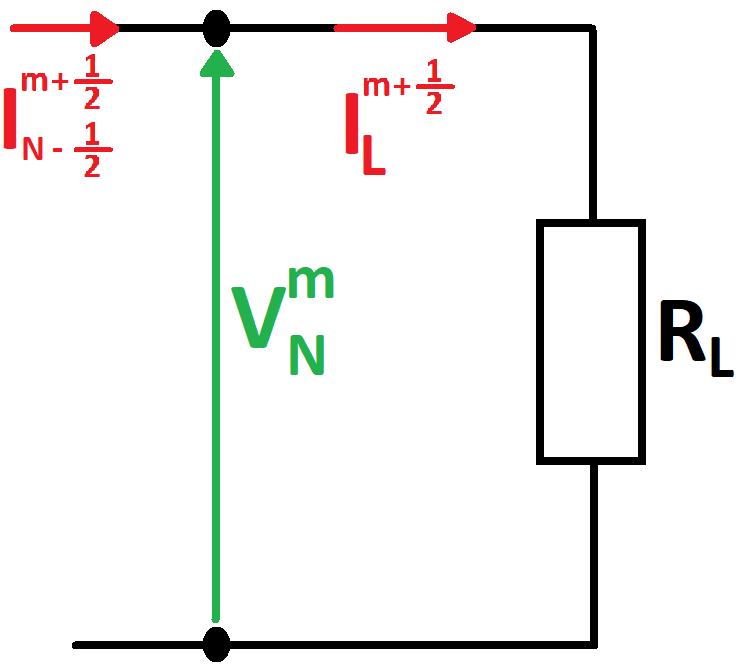
\includegraphics[scale=0.25]{BC2}

    The voltage update function becomes:
    \begin{equation}
        V^{m+1}_{N} = V^{m}_{N} + \frac{2\Delta t}{C\Delta z}\left(I^{m+\frac{1}{2}}_{N-\frac{1}{2}} - I^{m+\frac{1}{2}}_{L}\right)
        \label{BC2}
    \end{equation}
    Kirchoff's voltage law in discretized form states that
    \begin{align}
        I^{m+\frac{1}{2}}_{L} & = \frac{V^{m+\frac{1}{2}}_{N}}{R_{L}}\\
        & = \frac{V^{m}_{N}+V^{m+1}_{N}}{2R_{L}}
        \label{IL}
    \end{align}
    Subsituting \ref{IL} in \ref{BC2} and using the same relations as for $z=0$ and the new defined constant $\tilde{R}_{L} = \frac{R_c}{R_L}$ yields, 
    after some rearrangements:
    \begin{equation}
        V^{m+1}_{N} = C_{3}V^{m}_N + C_{4}\tilde{I}^{m+\frac{1}{2}}_{N-\frac{1}{2}},
    \end{equation}
    where
    \begin{align}
        C_{3} & = \frac{(1-\alpha\tilde{R}_{L})}{1+\alpha\tilde{R}_{L}},\\
        C_{4} & = \frac{2\alpha}{1+\alpha\tilde{R}_{L}},
    \end{align}
    are two dimensionless constants.
\end{itemize}

\end{multicols}




\end{document}